\setAuthor{Jaan Kalda}
\setRound{piirkonnavoor}
\setYear{2024}
\setNumber{G 4}
\setDifficulty{4}
\setTopic{TODO}

\prob{Galileo termomeeter}
\begin{wrapfigure}{r}{0.27\textwidth}
  \vspace{-25pt}
  \begin{center}
  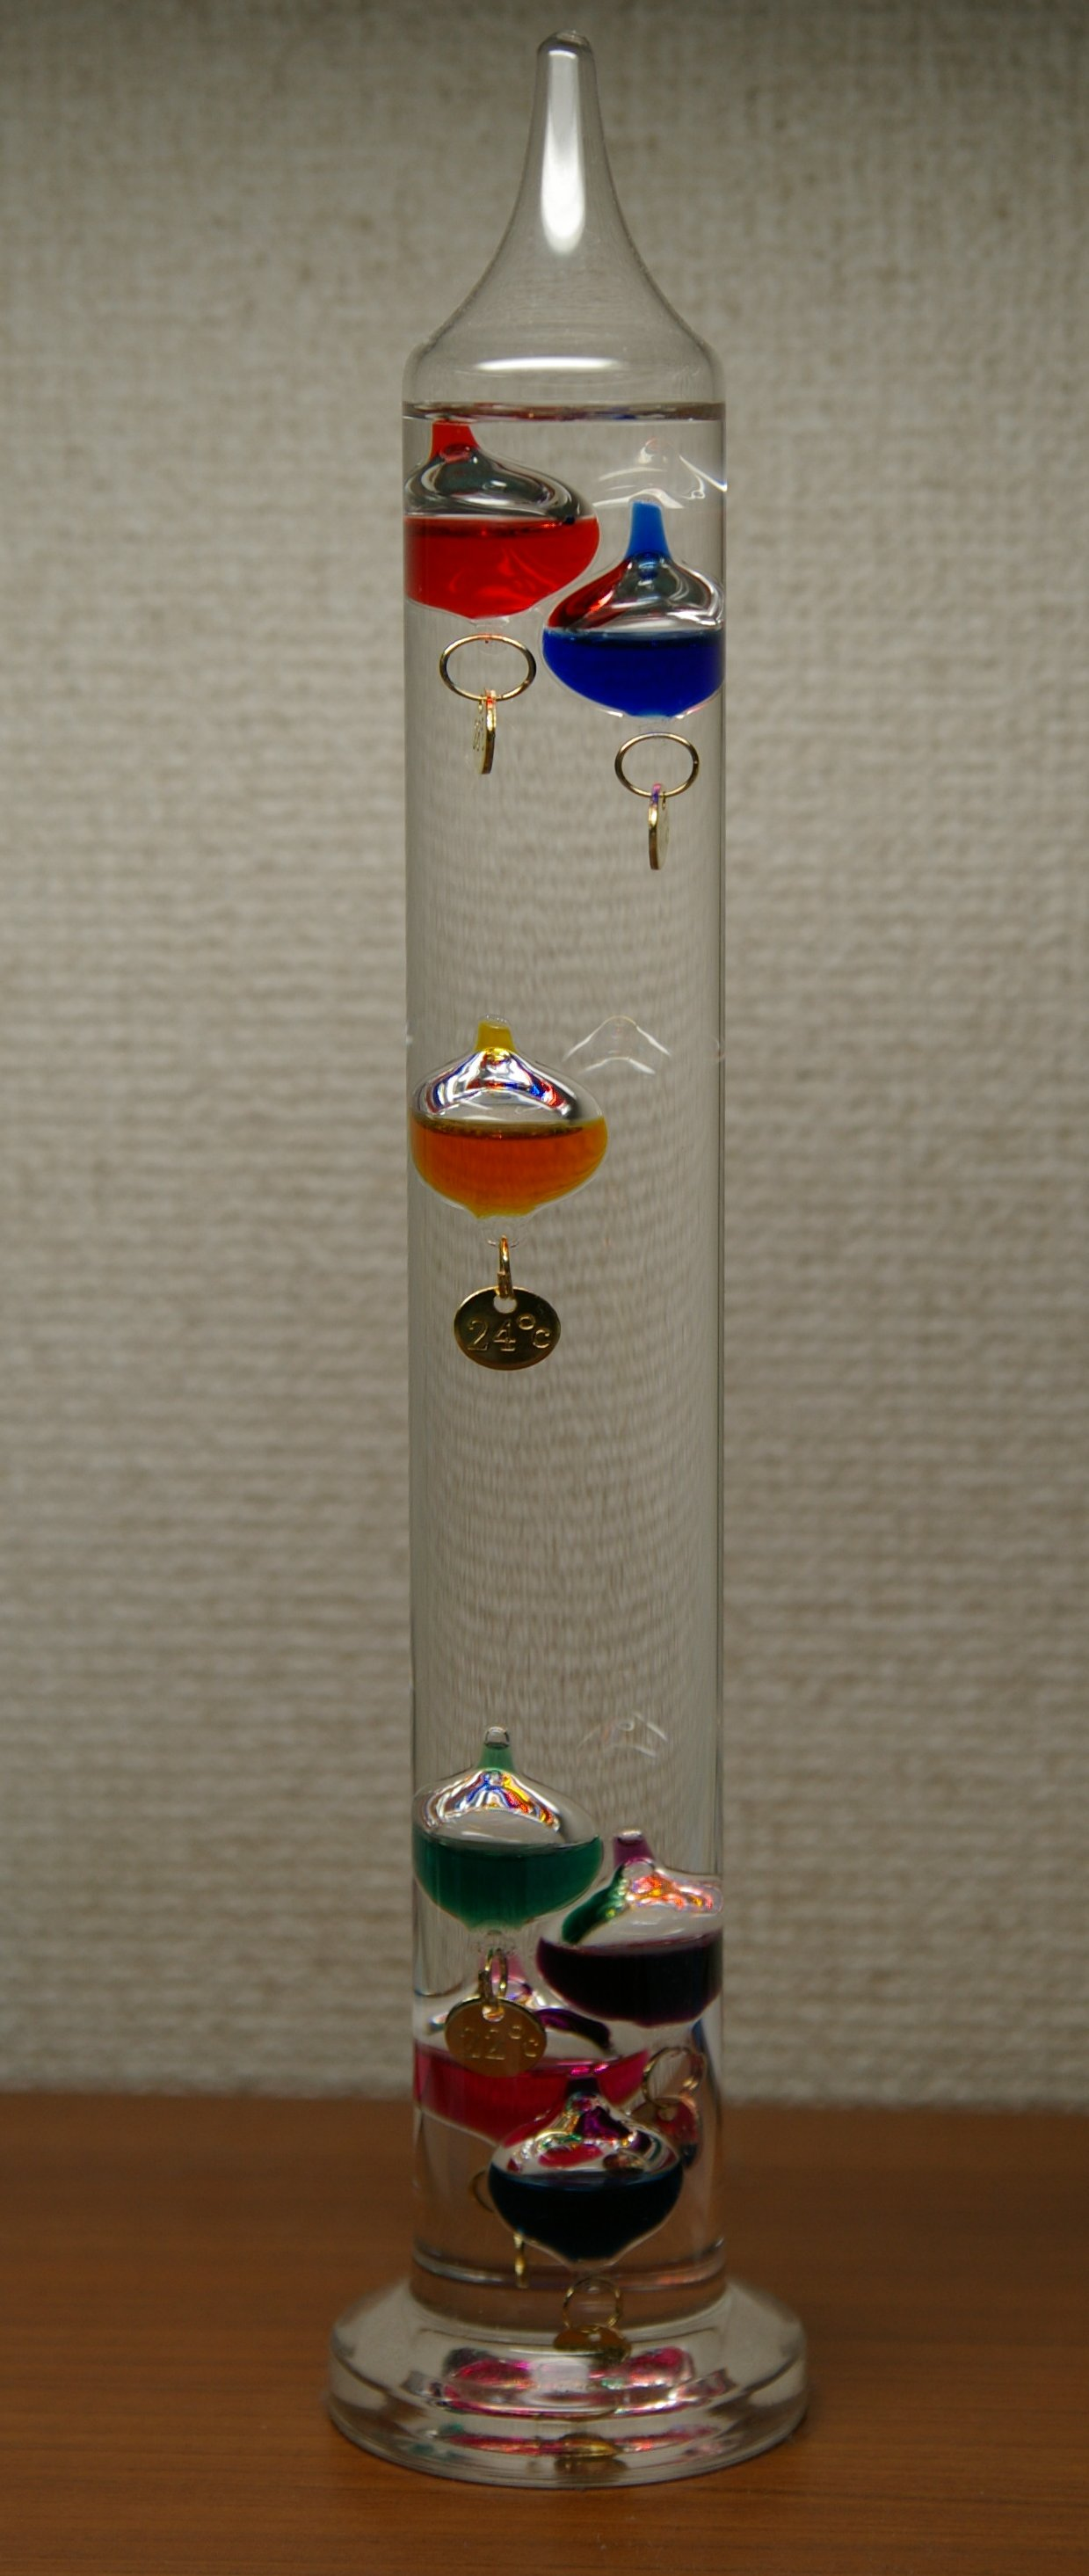
\includegraphics[scale=0.14]{2024-v2g-04-yl.jpg}
  \vspace{-20pt}
  \end{center}
\end{wrapfigure}

Galileo termomeetris (vt foto) hõljuvad vees erineva massiga, kuid sama ruumalaga kuulikesed (see ruumala arvestab nii kuulikest kui ka sinna külge kinnitatud sildikest). Kuulikeste keskmine tihedus on väga lähedane vee tihedusele. Et vee tihedus sõltub temperatuurist, siis sõltuvalt temperatuurist võib kuulike tõusta nii pinnale kui vajuda põhja. Kui teatud kuulike hõljub anuma põhja ja veepinna vahel, siis on temperatuur võrdne selle kuulikese külge kinnitatud sildil näidatud temperatuuriga. Silti $\SI{20}\celsius$ kandva kuulikese kogumass (koos sildikesega) on $m_1=\SI{20.000}{\g}$; milline on silti $\SI{22}\celsius$ kandva kuulikese mass? Vee ruumpaisumistegur on $k=\SI{2.1e-4}{\per\celsius}$, kuulikeste ruumpaisumistegur on sellest hulga väiksem. \textit{Vihje:} Ruumpaisumistegur kirjeldab ruumala suhtelist suurenemist temperatuuri tõusmisel $\SI{1}{\celsius}$ võrra, valemkujul: $\frac{\Delta V}{V} = k\Delta T$.


\hint

\solu
Olgu kuulikese koguruumala $V$; sellisel juhul vee tihedus 20 kraadi juures $\rho_1$ rahuldab tasakaalutingimust $\rho_1V=m_1$ \p{1}. Sarnase seose saame 22-kraadise kuulikese kogumassi jaoks, $m_2=\rho_2V$, kus  $\rho_2$ tähistab vee tihedust 22 kraadi juures \p{1}. Ühikmassi vee ruumala 20 kraadi juures on $V_1=1/\rho_1$ ja 22 kraadi juures ---  $V_2=1/\rho_2$ \p{1}. Teisest küljest $V_2=V_1(1+k\Delta T)$, kus $\Delta T=\SI 2\celsius$ \p{1}. Seetõttu $\rho_2=1/V_2=1/[V_1(1+k\Delta T)]=\rho_1/(1+k\Delta T)$ \p{1}. Et  esimese kahe valemi põhjal $m_2=\rho_2V=m_1\rho_2/\rho_1$ \p{1}, siis  $m_2=m_1/(1 + k\Delta T) $ \p{1}. Numbriliselt saame $m_2= \SI{19.9916}g$ \p{1}.
\probend